\documentclass[letterpaper]{article}
\usepackage{amsmath,amssymb,appendix,color,etoolbox,
  graphicx,index,listings,lscape,natbib,url}

\usepackage{mathpazo} % math & rm
\linespread{1.05}        % Palatino needs more leading (space between lines)
\usepackage[scaled]{helvet} % ss
\normalfont
\usepackage[T1]{fontenc}

\newcommand\figref[1]{Figure \ref{fig:#1}}
\newcommand\tabref[1]{Table \ref{tab:#1}}
\newcommand\code[1]{\texttt{#1}}
\newcommand\pipe[0]{\;|\;}
\newcommand\st[0]{\;\mathrm{s.t.}\;}
\newcommand\startappendix{\appendix\appendixpage\addappheadtotoc}

\newcommand\imgfig[4]{
\begin{figure}[h]
  \centering
  \includegraphics[scale=#2]{figures/#1}
  \caption{#3}
  \label{fig:#4}
\end{figure}}

\definecolor{gray}{gray}{0.95}

\lstset{
  language=Python,
  basicstyle=\footnotesize\ttfamily,
  numbersep=5pt,              
  tabsize=2,                  
  extendedchars=true,         
  breaklines=true,            
  stringstyle=\ttfamily, 
  showspaces=false,      
  showtabs=false,        
  xleftmargin=17pt,
  framexleftmargin=17pt,
  framexrightmargin=5pt,
  framexbottommargin=4pt,
  backgroundcolor=\color{gray},
  showstringspaces=false 
 }

\title{Stable Flight and Object Tracking with a Quadricopter using an
  Android Device}
\author{Benjamin Bardin \and William Brown 
  \and Dr. Paul Blaer}

\begin{document}

\maketitle

\begin{abstract}
  We discuss a novel system architecture for quadricopter control, the
  Robocopter platform, in which the quadricopter can behave
  near-autonomously and processing is handled by an Android device on
  the quadricopter. The Android device communicates with a laptop,
  receiving commands from the host and sending imagery and sensor data
  back. We also discuss the results of a series of tests of our
  platform on our first hardware iteration, named Jabberwock.
\end{abstract}
\tableofcontents
\pagebreak

\section{Motivation}
\subsection{Objectives}
We approached this project with three goals in mind: stable flight,
telepresence with an Android device, and simple blob tracking for the
helicopter. For stable flight control, we wanted a system that could
maintain a hovering state within a narrow radius of a given point (our
target radius was ten feet), and could respond to commands sent from a
host computer. For telepresence, we wanted to be able to visualize the
Android device's location, orientation, acceleration, and velocity in
real-time, as well as receive a video stream that compensated for
network latency and low bandwidth. Finally, we wanted a system that
would be able to grossly track objects on the ground to follow them
using a naive color-matching algorithm implemented on the Android
device.

\subsection{Potential Applications}
The applications for this platform are numerous; for example, the
Robocopter platform could be invaluable as a remote surveillance
tool. One application for which autonomous quadricopters are already
being used is disaster relief: the EU is currently funding the AWARE
project \citep{aware}, whose goal is to create cooperative
quadricopters to survey disaster sites and bring in light loads, such
as dried food or medicine. The Robocopter platform is capable of doing
much of what the AWARE quadricopters can do, but at much lower cost;
since the platform requires only an Android device and about four
hundred dollars of hardware, they can be manufactured extremely
cheaply.

\subsection{Progress}
At the time of writing, we have attempted stable flight but have
ultimately failed. We performed multiple outdoor tests, but have yet to
see any sort of stability. We discuss why we think this is the case in
Section \ref{sec:cls}. In one of the tests, the Jabberwock completely
lost control and, instead of flying, attempted to dig a hole. In this
test, the chassis was severely damaged. The electronics, thankfully,
escaped unscathed. This fall, we plan on rebuilding the chassis and
returning to our tests.  We will implement the platform changes
discussed in Section \ref{sec:cls} to prevent the catastrophic failure
we experienced with the platform, as outlined in this paper.

\subsection{Future Goals}
We have discussed various uses of the Robocopter platform. Currently,
we would like to implement a more robust blob tracking to allow the
helicopter to track objects as they move. Currently, since the blob
tracking is performed via color matching, changes in lighting or
orientation of the tracked object can result in a lost lock. Tracking
based on something more robust, such as SIFT features, would make our
blob tracking perform much better.  We would also like to implement
dynamic panorama creation, in which the helicopter performs a series
of predefined acrobatics to take photos which cover a solid angle of
180 degrees. From this, we can create a panorama from the helicopter's
current location; such birds-eye panoramas would be unusual, if not
unique, and would be both creatively and technically interesting to
generate.

\section{Pilot Android Application}
\label{sec:pilot}
The Pilot program has two core functionalities. The first is the
actual robotic control of the quadrocopter itself; the second is
communication with the control server. The parallel processing
required in these distinct tasks is complicated by the performance
requirements of the program. Flight control processing must take place
in real time -- or an extremely close approximation. Communication
with the control server, on the other hand, yields priority to flight
control. Consequently, a great deal of effort went into prioritizing
inter-thread communications and access of shared data. For flight
control algorithms, blocking on locked data is unacceptable, since
timely performance is essential; instead of blocking, they will use
the most recent, locally stored version of the data requested. For
communication algorithms, accessing flawed data is unacceptable; the
control server must not receive out-of-date information portrayed as
current.

\subsection{Flight Control}
Flight control itself is divided into two main components: navigation
and guidance.
	
\subsubsection{Navigation}
Navigation determines a desired velocity vector for the quadrocopter.
In ``manual'' mode, it simply accepts this vector from the control
server. In ``autopilot'' mode, or when the connection is lost, autopilot
subroutines determine the desired velocity vector. It's determination
is based on two factors. The first is its current location. The second
is either previously transmitted autopilot instructions, or
pre-programmed safeties (for low power, bad network, etc.).

\subsubsection{Guidance}
Guidance takes the desired velocity from Navigation, and uses PID
loops to adjust individual motor speeds to achieve and maintain that
vector.  To improve the performance of the PID loop, the system is
transformed into an approximately linear one.  The transformation
accounts both for the quadratic relationship between motor speed and
thrust, and for changing effects of motor thrust as its orientation
changes.

\section{Server Software}
\begin{figure}[h]
  \centering
  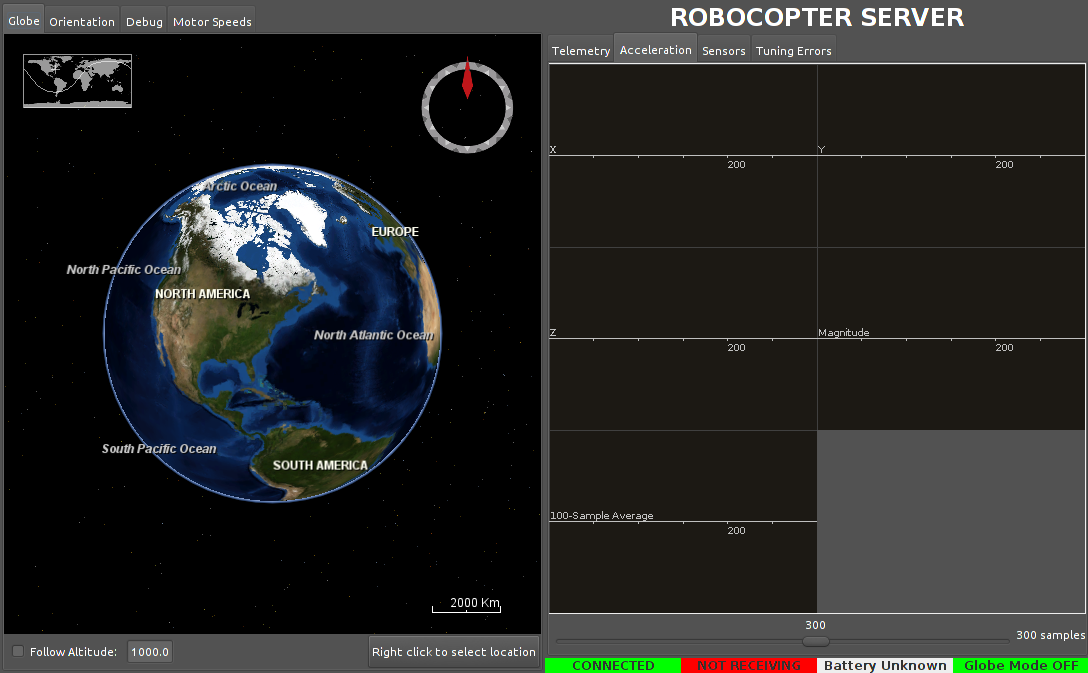
\includegraphics[scale=0.3]{figures/globe-screenshot}
  \caption{A screen capture of the chopper control software.}
  \label{fig:globe}
\end{figure}

\begin{landscape}
  \begin{figure}[h]
    \centering
    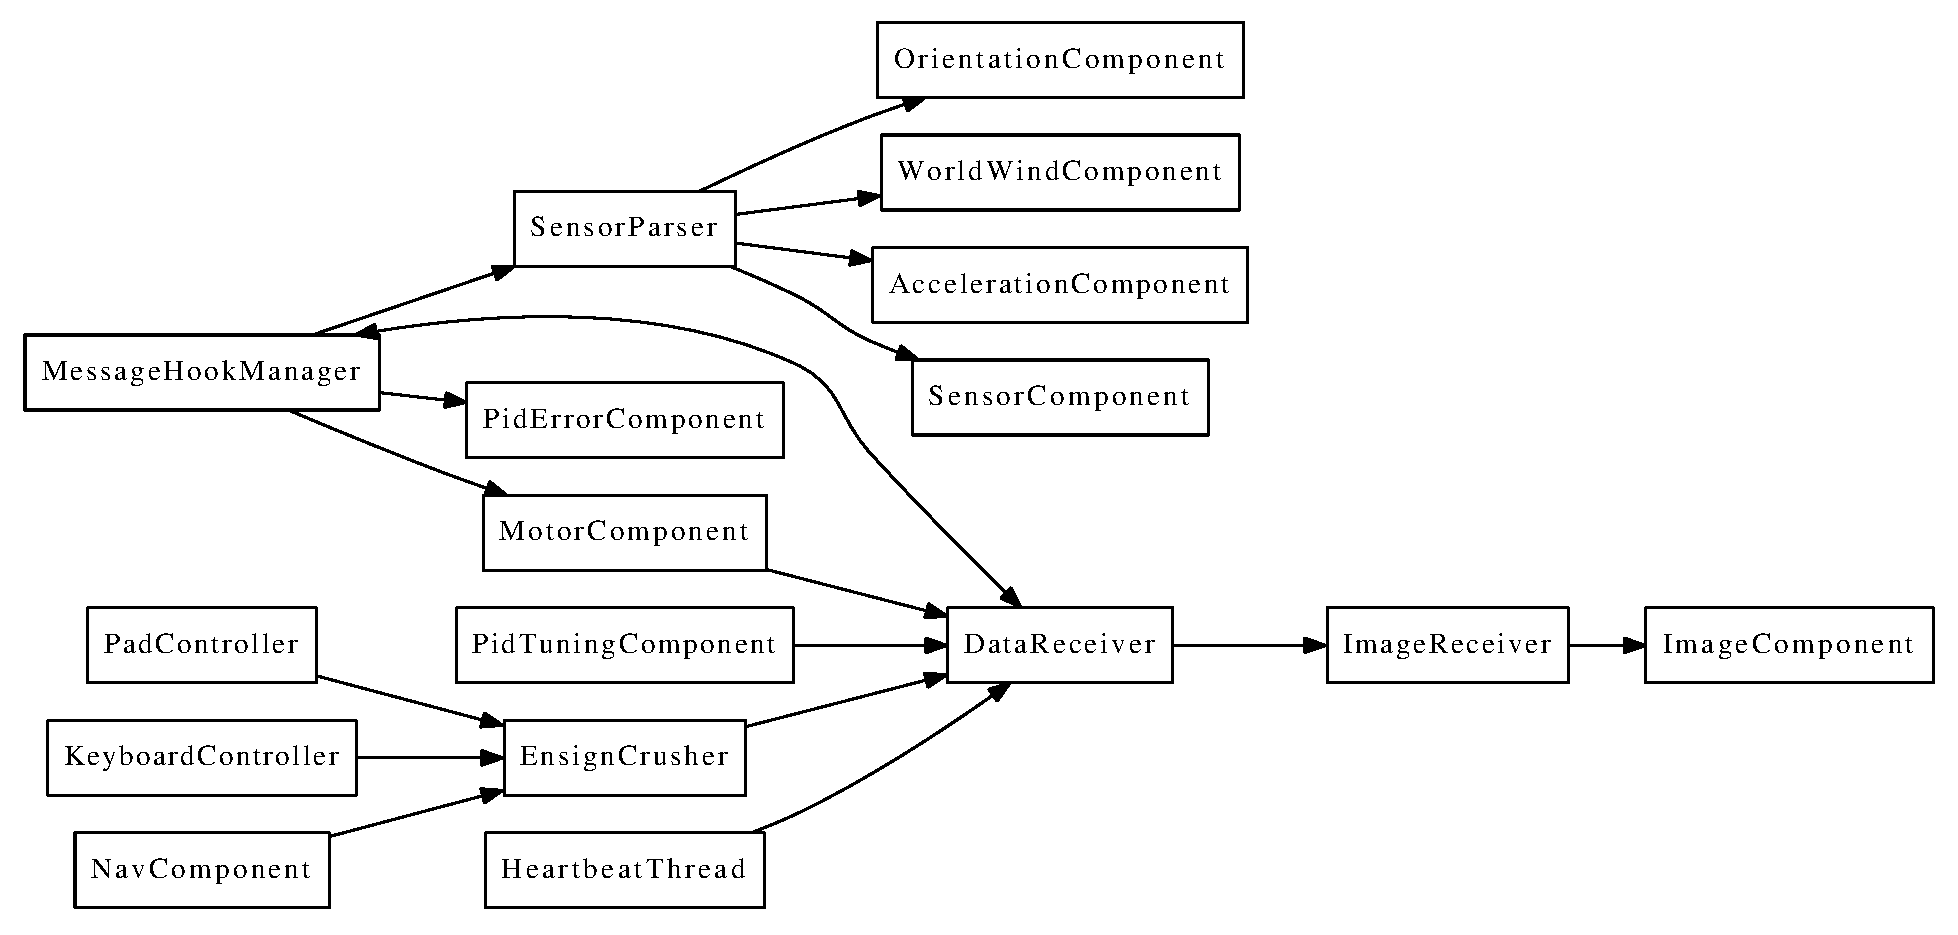
\includegraphics[scale=.5]{figures/hostarch}
    \caption{The architecture of the host system}
    \label{fig:hostarch}
  \end{figure}
\end{landscape}

The software is designed for two purposes: control and
telepresence. We have implemented a system which allows us to monitor
acceleration, orientation, temperature, location, and even magnetic
flux. We also are streaming video from the helicopter to the server
software, which is displayed in the UI. We have a control subsystem
that allows us to control the helicopter from a mouse-based system, a
keyboard-based system, or a Microsoft XBOX controller. 

The architecture of the system is shown in \figref{hostarch}.

\subsection{Message Handling}
Sensor readings from the phone are transmitted to the server using
very simple strings, as is described in Section \ref{sec:msgs}. These
are received and placed into a message queue which handles all
subsequent processing. The various components of the UI and backend
are all programmed as plugins to this message queue handler. Each
plugin registers a list of prefixes with the message queue -- these
define the messages that that plugin is capable of processing. For
example, the orientation component handles only messages with the
prefix ``ORIENT'', while the PID tuning component handles anything
that starts with ``GUID'' or ``NAV'' (for guidance and navigation,
respectively). The appropriate messages then get passed onto these
components who handle the messages themselves.

The message handler receives a huge firehose of information, and only
about 10\% of the plugins need to respond to any given message. In
early implementations, every plugin received every message, which
meant that about 90\% of the work on each message was useless. In
instrumenting early builds using VisualVM, we found that about 60\% of
the processing done by the sever was trying to handle each of the
messages, and often the queue would fill faster than it was
emptying. Two fixes improved this: the prefix-based handling (which
cut down on processor usage) and multithreaded plugins. Some of the
plugins were blocking the processing of later messages because the
plugins were given new messages synchronously -- switching to an
asynchonous update mechanism for some of the heavier plugins allowed
us to decrease latency in sensor readings and other easier-to-process
messages.

\subsection{Telepresence}
The main thing we tried to accomplish in designing the UI was to make
it as easy to understand what the helicopter was doing as possible,
and be able to access all of the data the Android platform was capable
of giving us. We also wanted it to be easy to detect error conditions
at a glance for faster operator response to emergencies.

We eventually decided that, for many sensors, graphing them was the
most intuitive way to do this. To graph them, we rolled our own
graphing package (which was later released as SimpleGraph, a standalone
Java line graph library). For three, however, there were more
intuitive ways of displaying our data. 

For orientation, we used a 3D representation of the helicopter that
accurately mirrors the orientation of the actual phone, which is
easier to read than trying to apply three rotations in your head. We
used the Java3D\footnote{https://java3d.dev.java.net/} game library
for this, because it was the most resource-efficient in our testing. 

For location, we chose to mimic the Google Earth interface and used
NASA's World Wind\footnote{http://worldwind.arc.nasa.gov/java/}
mapping software. This is an extraordinarily powerful library, and the
only one we could find of its kind. Though poorly documented, it is open
source and very easy to use.  Consequently, we dropped it into our UI
quickly and seamlessly. 

The last visualization we used was a very simple top-down view of the
helicopter for the motor speeds, in which each ``motor'' is given a
color from red to green, denoting the current speed of the motor.

\section{Communication}
Communication is composed of two main components: telemetry and
commands/data. Each is relayed on separate ports, since commands must
be relayed as synchronously as possible and telemetry will be
asynchronous.

\subsection{Telemetry}
The telemetry modules continuously run the Android's preview
functionality, at 5fps.  Each frame is saved to a buffer as it is
available, overwriting the previous frame.  When the Android has
finished sending one frame to the control server, it immediately
copies the buffer and starts sending the frame.  The result is real
time telepresence, at approximately two to four fps and a lag of
less than one second.

\subsection{Commands and Data}
Commands and data are relayed in the form of strings over standard
Java sockets. When the connection is lost, the Android device
immediately tries to reconnect, continuing to do so indefinitely.
While the connection is lost, autopilot is enabled and the
``communication lost'' pre-programmed instruction set is engaged.

\subsection{Message Formats}
\label{sec:msgs}
‏Messages between the Android and the control server are sent as
strings, delimited by colons. The strings from the control server --
commands -- contain the instruction itself, prefixed by a sequence of
meta-data describing the instruction. Similarly, data from the Android
device contain not just the data, but also a prefix tag describing the
data. This enables somewhat efficient analysis on each end: messages can
be routed only to those components that are registered to process a
given prefix tag.  Messages are not transmitted directly between the
Android device and the control server. Instead, they are routed through
a separate, dedicated broker server. This enables the control server
itself to operate easily from different IP addresses, and hence from
various locations. It also allows for easy logging and playback of
sessions -- the broker server logs all data and commands, and can replay
a session later for analysis.

\section{Jabberwock}
A list of parts used is supplied in Appendix \ref{tab:parts}.

\subsection{Design of the Chassis}
The chassis design has fluctuated the most over the process. While the
software stack was fairly well thought out early on, we wrote it to be
hardware-independent. At first, the plan was to use a kit chassis and
buy our own components, as this would mean that all of the components
would be guaranteed to work together. However, as time went on, we
realized that the added cost of a robust chassis was higher than the
value we would get out of it, and we decided to build our own.

Using a 3D printer, we were able to print whatever plastic parts we
desired out of ABS plastic. ABS is a rigid and strong plastic -- it is
best known for being the raw form of a Lego brick -- and is very cheap
to buy in large quantities. Jabberwock was printed on a Makerbot that
is capable of printing objects up to 10cm by 10cm by 13cm: it
wasn't large enough to build the entire helicopter in one go. Our
design, therefore, had to account for the fact that no individual
custom-made part could exceed these dimensions.

\begin{figure}[htb]
  \centering
  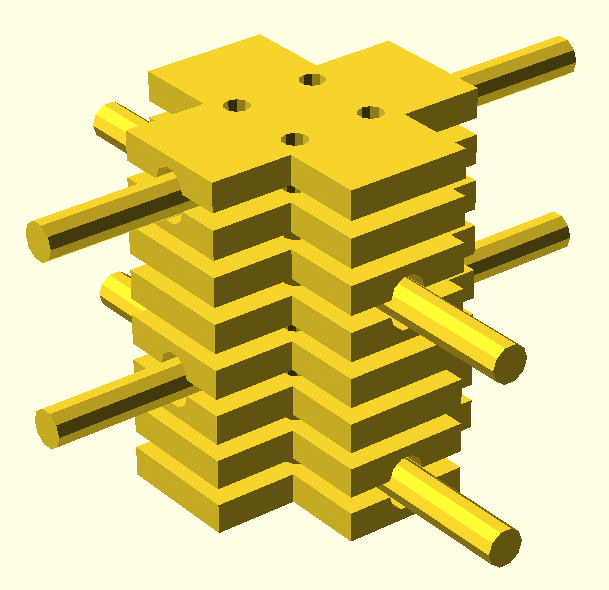
\includegraphics[scale=0.4]{figures/brock_assembly}
  \caption{The center assembly upon which the electronics and Android
    device are mounted.}
  \label{fig:brock}
\end{figure}

\begin{figure}[htb]
  \centering
  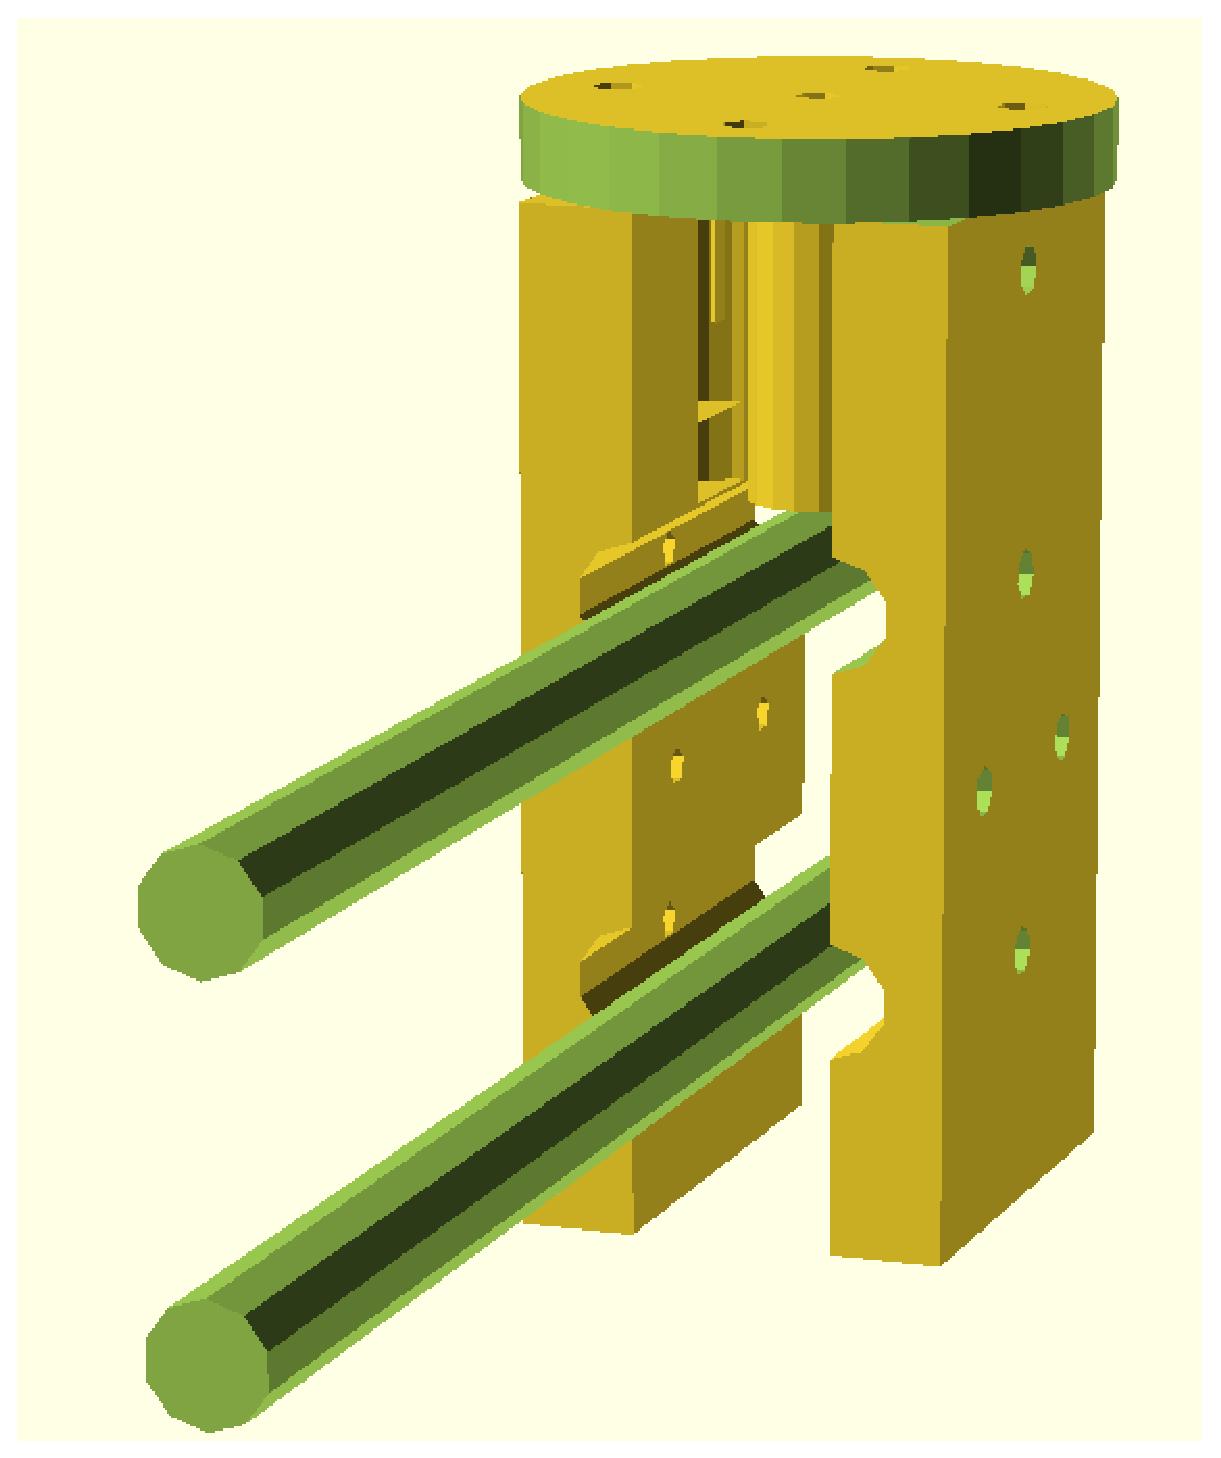
\includegraphics[scale=0.4]{figures/fred}
  \caption{A motor mount on the end of a pipe.}
  \label{fig:fred}
\end{figure}

We opted for a design that is slightly different from most
commercially-available quadricopter designs, for both pragmatism and
strength. Our design features a large block in the middle made
of sandwiched layers, each of which holds a narrow-gauge brass pipe in
place. A rendering of this component can be seen in
\figref{brock}. These brass pipes extend 25 cm out either side of this
center block. On the end of each pipe is a motor unit, consisting of
two sandwiched ABS pieces that attach the motor to the pipe. This can
be seen in \figref{fred}.

The first and last layer of the center block each have eight mounting
holes with a captive nut locked in between the outer layer and next
layer. This allows us complete modularity in terms of hardware
attachments without ever having to reprint -- all we must do is
make sure new components are compatible with the mounting screws already
built in, and we can hotswap our hardware easily.

\subsection{Electronics Design}
In designing the electronics, we went for as much redundancy as
possible, and only used parts that had ratings at least 50\% over our
estimated needs. We estimated that the helicopter would have a weight
of approximately 1 kg (actual weight was slightly higher) so each
motor-propeller pair needed to be rated to
carry at minimum 500 grams. In addition, we wanted to be able to put
different payloads on the helicopter in the future (if we wanted to
mount a video camera, for example) so we ended up using
motor-propeller pairs that are capable of a very large range of
possible thrusts, from around 50 grams to about 1.5 kg per motor. In
later testing, we learned that the helicopter was neutrally buoyant
when all motors were set to about 30\%.

For our control hardware, we chose to use an Arduino because we had
experience coding for the Arduino platform, and because it provides many
libraries that are helpful for motor control and sensor
readings. While the sensor reading libraries were not used for
Jabberwock, in later iterations we plan may use rangefinding sensors
for landing and three-dimensional map creation, so we wanted to ensure
we had the capability to hook that in to the existing system.

We chose our other parts based on online reviews and price. One of our
goals was to keep this project as cheap as possible for two reasons.
Firstly, we wanted to be able to pay for the thing, and secondly, we
were interested in seeing just how cheaply this could be done. In the
end, we managed to keep the cost low -- \$440 after tax and shipping.

We did make one fairly nonconventional decision in terms of
electronics design. While many designs use only one battery to power
the entire system, we chose instead to have four batteries -- one for
each motor. This has the disadvantage that we have to monitor four
battery charges instead of one, the wiring is slightly more complex,
and the batteries can discharge at different rates. However, having
the four batteries has one distinct advantage: increased
longetivity. Having all four batteries means we can stay flying for
longer, which is a clear advantage.

\section{Blob Tracking}
We would like the Robocopter platform to be able to track gross
objects based on color. To that end, this semester, we implemented a
blob tracking algorithm that can run on both Android and a standard
JVM. The algorithm is capable of image segmentation, labelling and
object motion tracking. The architecture of this algorithm is outlined
in \figref{blob}.

\imgfig{blob}{.5}{Architecture of the blob tracking system}{blob}

\subsection{Algorithm}
\subsubsection{Image Segmentation}
For image segmentation, we used an adaptive algorithm that segments an
image based on a color and a threshold. There is a matching phase, and
then a learning phase. In the matching phase, the segmenter takes an
RGB image and outputs a binary image, representing color
matches. Treating color as a 3-vector, the output image is defined by
\ref{eq:segment}, where $O$ is the output image, $I$ is the input
image, $C$ is the target color and $t$ is the threshold. After the
output is computed, it iteratively expands this field. Each iteration
passes through the image, activating any pixel that has a neighbor who
is active. The number of expansion passes is configurable, but we
found the best results with a single expansion pass.

\begin{equation}
  \label{eq:segment}
  O_{(x,y)} = \left\{ 
    \begin{array}{rl}
      1 &:\; || I_{(x,y)} - C || < t \\
      0 &:\; \mathrm{otherwise}
    \end{array} \right.
\end{equation}

The learning phase happens after labelling and connected component
analysis. After connected component analysis, the system has a
best-guess for which blob in the segmented image represents the object
which we are tracking. We find the mean color within that blob, and
take the mean of that color and our current color. The resulting
midpoint is set to be the new target color. This adaptation ensures
that moderately slow changes in lighting will not effect the
performance of object tracking.

\subsubsection{Image Labelling}
We used a standard two-pass algorithm to find the connected components
in the result of segmentation that uses 4-connectivity to define pixel
adjacency. The first pass of this algorithm labels each pixel based on
whether its neighbors above and to the left are set. It also records
when there is a equivalence collision (i.e., when both the pixel above
and to the left are labelled, but they have different labels). In this
case, it adopts the label of the lowest value (the parent label) and
records the two labels in an equivalence table. The second pass then
iterates over the image, replacing child labels with parent
labels. The result is a list of \code{Area} objects, each of which
contains a centroid and size.

\subsubsection{Connected Component Analysis}
The result of segmentation and labelling usually returns multiple
labelled areas. The analysis step attempts to determine which of the
areas is the one which we are tracking. Since we were unsure of the
rate at which the Android device would be capable of processing
images, we wanted to make this step independent of location. If the
phone could only process a few frames per second, it is possible that
the tracked object could have moved significantly between frames. We
could not, therefore, make the assumption that the closest area to the
area we detected last was our target. Instead, we made the assumption
that the size of the object in the frame would be relatively
invariant. Based on this assumption, we chose to take the blob whose
area was most similar to the previously detected area as our target.

\subsubsection{Reaction and Tracking}
Once we have the in-frame location, we translate this to coordinates
centered on the origin. For example, if the centroid of an area was
detected to be in the center of the image, the resulting coordinates
would be (0, 0). We then translate this into a navigation 3-vector, in
which the Z-component is zero, and the X- and Y-component are the
corresponding values in these coordinates, multiplied by a scaling
factor. This is then passed to \emph{Navigation}.

\subsection{Performance and Results}
Since we were unable to maintain stable flight, we were unable to test
the reaction and tracking step. However, we found that the tracking
worked well. In lighting-invariant conditions, it was able to track an
object as either the object or the camera was moved. To test it, we
set up the blob tracking to run on a laptop while receiving imagery
from the Droid. The laptop was able to segment these images faster
than it received them from the Droid, which places a lower bound of 5
Hertz on the frequency of which this algorithm is capable. Further
testing is needed before we can know how fast the algorithm is capable
of running on an Android device, especially while said device is
running the rest of the Robocopter system.

\section{Testing}
\subsection{Pilot Application Testing}
For budget reasons, we did much of the initial Pilot development on
the android emulator.  As one might imagine, this proved to be a poor
platform for developing robotic control software.

The emulator does not, in fact, actually emulate many hardware
functions very well.  The camera functionality does not properly
implement several guaranteed methods: for example, a
\code{Camera.parameters} object on which
\code{getSupportedPreviewSizes()} is called returns null, though the
API specifies that a list is guaranteed.  Less culpably, calling most
bluetooth-related methods will crash the program on the emulator.

A persistent developer can code around these drawbacks, testing other
aspects of the program on the emulator.  More damaging is the speed at
which the emulator runs: it is very, very slow.  This is hardly
unexpected, but running moderately complex control algorithms at even 10
Hertz quickly becomes untenable.

Another hazard we noticed was more subtle.  On the emulator, many
sensors are not implemented, and those that are return constant
values.  The orientation sensor is an instance of the former; the
acceleration sensor one of the latter.  On a real phone, this is
obviously not the case, and many bugs in the software only became
apparent after migrating from the emulator to the Droid.  For
instance, the emulator always read the azimuth value as zero:
consequently, it never actually executed a coordinate transformation
of the velocity vector from the absolute frame to the relative frame.
On the emulator, the two were the same; on the Droid, they literally
never are.  This is a crucial piece of code that was not properly
tested for quite some time.

\subsection{System Testing}
\subsubsection{Systematic Delays}
Initially, we encountered a substantial delay in sending motor speeds
from the Pilot program to the Arduino.  After some testing, we
determined that the source of the delay was not, in fact, in our code,
but rather in the android inter-application messaging system.  The
published Amarino library runs a service -- \code{AmarinoService} --
to interface applications on the phone to the Arduino over bluetooth.
Applications send messages by broadcasting a system-wide \code{Intent}
object, which is sent to \code{AmarinoService}, processed, and
transmitted over bluetooth.  Since our control loop runs at 10 Hertz
and submits 4 motor values per loop, we were broadcasting system-wide
\code{Intents} at the rate of 40 Hertz.  This proved to be too much
for Android, which could not process the \code{Intent}s nearly fast
enough.

\imgfig{motor1}{.5}{Actual motor speeds vs. broadcasted motor speeds}{motor1}

A graph of desired versus actual motor speeds is shown in
\figref{motor1}. The red line indicates desired motor speeds, as
determined by the \code{Guidance} object, calculated in real time.
The green line indicates the time at which those commands were
actually sent over bluetooth by the \code{AmarinoService}.  The above
graph indicates not just a delay between the two, but an increasing
delay, suggesting an Android system queue to which elements were being
added faster than they were being removed.

We resolved this problem by bypassing the Intent-broadcast system
entirely.  In fact, we spliced the entire Amarino application into our
own.  When all components were run in the same JVM, we could easily
access the AmarinoService explicitly from Pilot and process messages
directly, instead of waiting for Android to resolve the broadcasts. A
similar graph to the one in \figref{motor1} is shown in
\figref{motor3}; \figref{motor3}, though, shows the results of this
modification.

\imgfig{motor3}{.5}{Actual motor speeds vs. broadcasted motor speeds,
  post-modification}{motor3}

While perhaps inelegant, this solution worked quite well.  The
convergence between \code{Guidance} and \code{AmarinoService} is
approximately perfect.

\subsubsection{Control loop stability}
\label{sec:cls}
After actual testing, it appears that the hardware limitations of the
Droid may preclude stable control of such a complex system.  The
orientation sensor on the Droid, even at its fastest setting, only
registers new values at ever 100ms or so (this delay is not
consistent).  Consequently, there is no purpose in running the PID
control loop at faster than 10hz.  However, the quadricopter loses
stability in well under a second.  The shift from ``stable'' to
``irrecoverably unstable'' can occur in as few as 3 or 4 tenths of a
second--and therefore only 3 or 4 iterations of the PID loop.  While
precise tuning might make control possible, even perfect tuning is
likely to yield poor control at best.  And obtaining even
``acceptable'' tuning at this point seems to be a futile endeavor.

\section{Future Improvements}

Moving forward, we have a number of enhancements planned that we think
will drastically improve stability.  Most importantly, we will be using
a newer Android device to pilot the quadricopter.  This device--an HTC
Evo 3D--possesses 4 times the processing power of the Droid, and
includes a gyroscope.  Between the two, we expect both more accurate
orientation readings and a faster sample rate.  We hope to run the
control loop at 33hz, instead of the current 10hz.

We will also implement changes to the control algorithms themselves.
First, we will not attempt to directly control the speed of the
quadricopter.  Instead, we will endeavor to control its orientation
directly, and control speed indirectly by altering target orientation.  
Second, as discussed earlier, PID control works best on a linear system.
Quadricopter mechanics, however, are far from linear.  Consequently, the
transformation from linear control variables--on which the PID loop
operates directly--to the non-linear motor speeds is of the utmost
importance.  Deeper analysis of the transformation we used on the
Jabberwock platform showed it to be quite flawed.  We have developed a
newer algorithm that we believe is far more accurate.

The chassis design will also undergo significant alteration, to improve
stability.  Each arm will be comprised of three brass rods, instead of
two.  Additionally, we will move the batteries from their current
positions on the arms to a new position under quadricopter's center of
gravity.  Between these two changes--and the software changes mentioned
above--we anticipate a hugely improved quadricopter system.

\newpage
\appendix
\section{Parts and Prices}
\label{tab:parts}
\begin{tabular}{llll}
  \textbf{Item} & \textbf{Supplier}
  & \textbf{Quantity} & \textbf{Price} \\
  Chassis Hardware & McMaster-Carr & N/A & \$32.60 \\
  Turnigy 2217 Brushless Motors & HobbyKing & 4 & \$14.04 \\
  Counterforce Propeller Pair & NG Hobbies & 5 & \$6.95 \\
  Arduino Microcontroller & SparkFun & 1 & \$29.95 \\
  Turnigy 15 Amp ESC Controller & HobbyKing & 4 & \$10.58 \\
  BlueSmirf Gold Bluetooth Modem & SparkFun & 1 & \$64.95 \\
  Turnigy 2200mAh 3S LiPoly Battery & HobbyKing & 5 & \$11.96 \\
  Arduino ProtoShield Layout PCB & SparkFun & 1 & \$16.95 \\
  HobbyKing Fast Battery Charger & HobbyKing & 1 & \$39.99 \\
\end{tabular}

\section{Code Repository}
A single github repository is used for version control of the server,
client and broker, as well as this essay.

http://github.com/haldean/droidcopter

\bibliographystyle{plainnat}
\bibliography{essay-spring}

\end{document}
